\section{Experimental Setup}

In this work, we simulated our evaluation environment entirely in software using the Cocoh \cite{Cocoh} C++ framework. Figure \ref{fig:simulation} shows an overview of what the simulation environment contains. At the top we have the accelerator implementation with its AAL interface, both modelled using Cocoh's API. At the bottom, we have the Cocoh's simulation runtime that bind the accelerator and the back-end host CPU simulator. Inside our host CPU simulator we modelled a QPI memory simulator which managed the shared memory space and served all the memory requests coming from the accelerator. In the current design we used a 1 GB shared memory space for holding the matrix and vertex data, including the output result from the accelerator. On the actual Xeon platform \cite{Intel-FPGA}, the shared memory space limit is 2 GB.

\begin{figure}[htbp]
\centering
\includegraphics[width=0.3\textwidth]{figures/simulation}
\caption{FlexGraph Simulation Environment}
\label{fig:simulation}
\end{figure}

\begin{figure}[htbp]
\centering
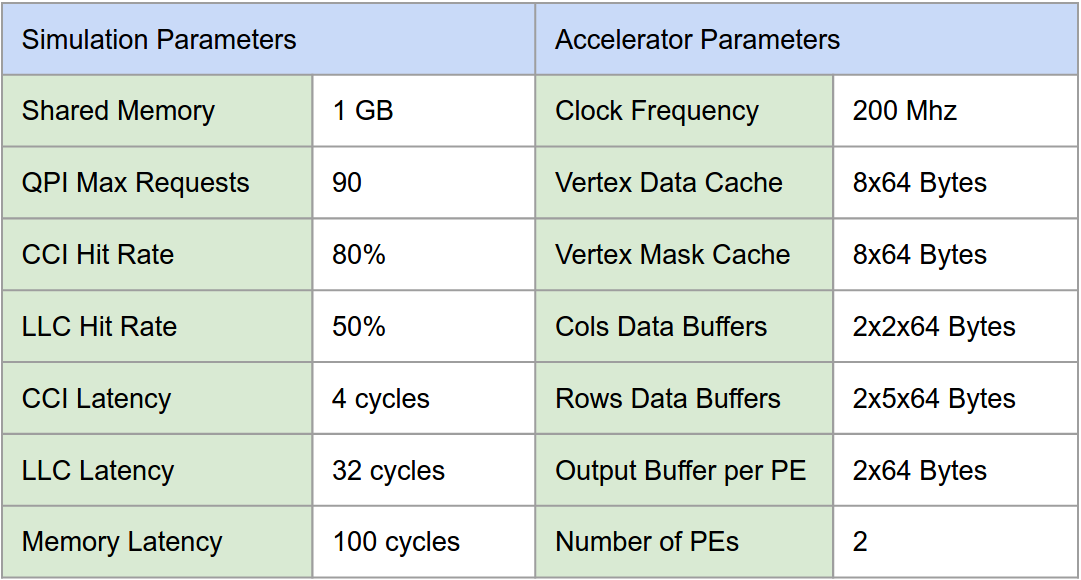
\includegraphics[width=0.4\textwidth]{figures/simulation_parameters}
\caption{FlexGraph Simulation Parameters}
\label{fig:simulation_parameters}
\end{figure}

\subsection{Intel QPI Simulation}
We simulated the Intel QPI memory transaction using an analytic model capturing the latency of memory transfers when the request hits local CCI \cite{CCI} cache or the host processor LLC. All outgoing memory requests from the accelerator to CCI take two cycles and the responses from CCI hits take another two cyles, giving a minimum round trip latency of four cycles for read requests. Figure \ref{fig:simulation_parameters} shows some configuration parameters we use for both the simulation and accelerator modelling.     

\subsection{Graph Datasets}

We used the Graph500 \cite{Graph500} synthetic datasets for our evaluation. We configured graph generator similar to GraphMat \cite{GraphMat} setting the default RMAT paramters (A=0.57, B=C=0.15 and D=1-A-B-C). We used five scaling factors for our graphs (6, 8, 10, 12, 14) with corresponding number of non-zero ranging from 1024 to 262,144 accordingly. These datasets are relatively small mainly due to simulation time constraints, but the setup could have supported up to a scaling factor of 20 (about 16,777,216 non-zeros). Due to time constraints we did not test any real world dataset, that will be discussed in our future work section. Figure \ref{fig:graph500_dataset} lists down the number of vertices and non-zeros for our dataset.

\begin{figure}[htbp]
\centering
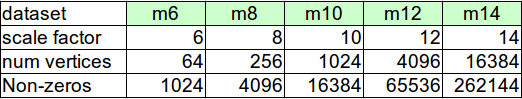
\includegraphics[width=0.4\textwidth]{figures/graph500_dataset}
\caption{Graph500 dataset}
\label{fig:graph500_dataset}
\end{figure}

\section{Results Analysis}

In this section, we discuss our evaluation results.

\subsection{Throughput Performance}

\begin{figure}[htbp]
\centering
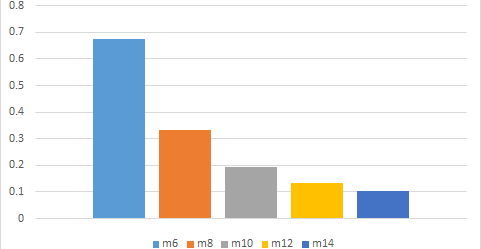
\includegraphics[width=0.5\textwidth]{figures/dual_core_perf}
\caption{FlexGraph Throughput Performance}
\label{fig:dual_core_perf}
\end{figure}

Figure \ref{fig:dual_core_perf} shows the throughput performance of the accelerator in GFlops. We estimated the performance using the following equation:
\[Perf = \dfrac{2 * nonzeros}{latency}\]
The performance varies from 0.67 Gflops to 0.1 Gflops as the size of the dataset increases. This result is comparable to our implementation of a similar kernel using the Altera OpenCL HLS, also showing similar performance degradation as the workload size increases. In prior work, GraphOps \cite{GraphOps} peak performance for their FPGA implementation was 0.18 GFlops with a graph size of 512K vertices, about x3 our throughput. The target platform has peak memory bandwidth is 6.0 GB/s, this shows that there is room for improvement. than We identified several optimization opportunities that we will discuss later in this section. 

\subsection{The Impact of Parallelism}

Figure \ref{fig:single_core_perf} shows the throughput performance of the accelerator in GFlops for a single-core system versus the dual-core implementation. We can see a considerable drop in performance (by almost half) across all datasets when a single processing element is executing. This is happening because there is much less memory level parallelism that can be exploited when a single core is running. In a dual-core system, the LSU receives a lot more memory requests from the processing element and has much less idle time when QPI is taking more cycles to return the blocks. When a processing element is stalled on a request, another may be able to make progress. We believe that increase the number of processing element beyond two will have a possible impact in performance for FlexGraph, possibly doubling the current throughput.

\begin{figure}[htbp]
\centering
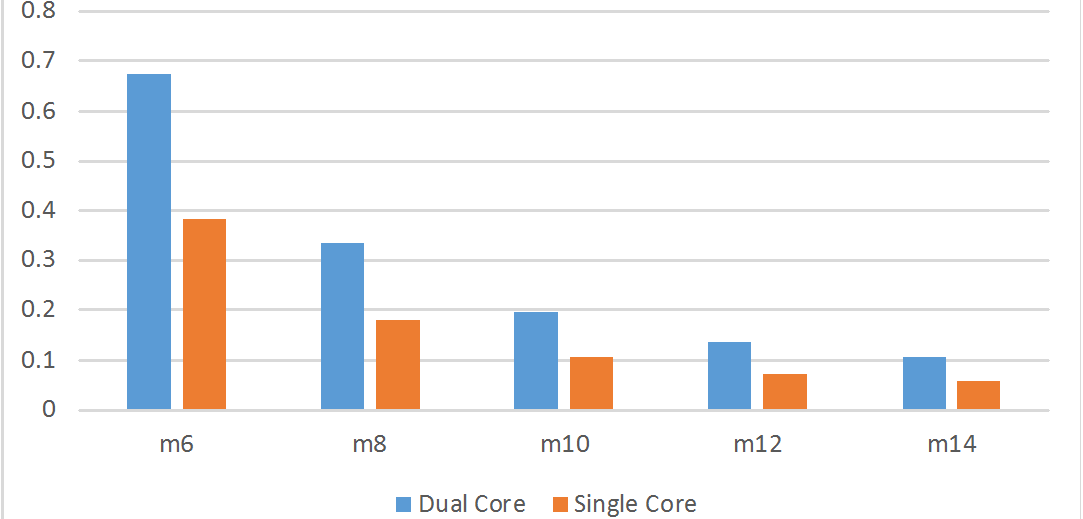
\includegraphics[width=0.5\textwidth]{figures/single_core_perf}
\caption{FlexGraph Single Core Performance}
\label{fig:single_core_perf}
\end{figure}

\subsection{The Impact of Memory Optimizations}

Figure \ref{fig:no_opts_perf} shows the accelerator performance with all memory optimizations disabled in GFlops. Once again the graph shows a similar performance degradation as the dataset size decreases. The memory optimizations give the accelerator an average performance speed-up of 45\%, which is significant considering the fact the the system is memory bound.

\begin{figure}[htbp]
\centering
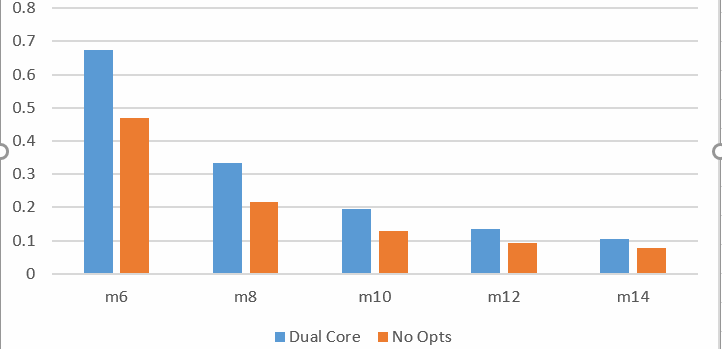
\includegraphics[width=0.5\textwidth]{figures/no_opts_perf}
\caption{FlexGraph Performance with memory optimizations}
\label{fig:no_opts_perf}
\end{figure}

\subsection{Summary Discussion}    

\begin{figure}[htbp]
\centering
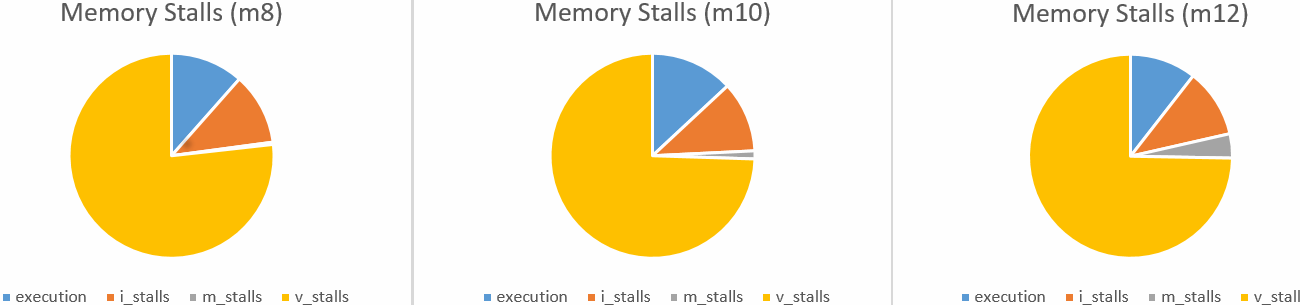
\includegraphics[width=0.5\textwidth]{figures/memory_stalls}
\caption{FlexGraph Memory Stalls}
\label{fig:memory_stalls}
\end{figure}

\begin{figure}[htbp]
\centering
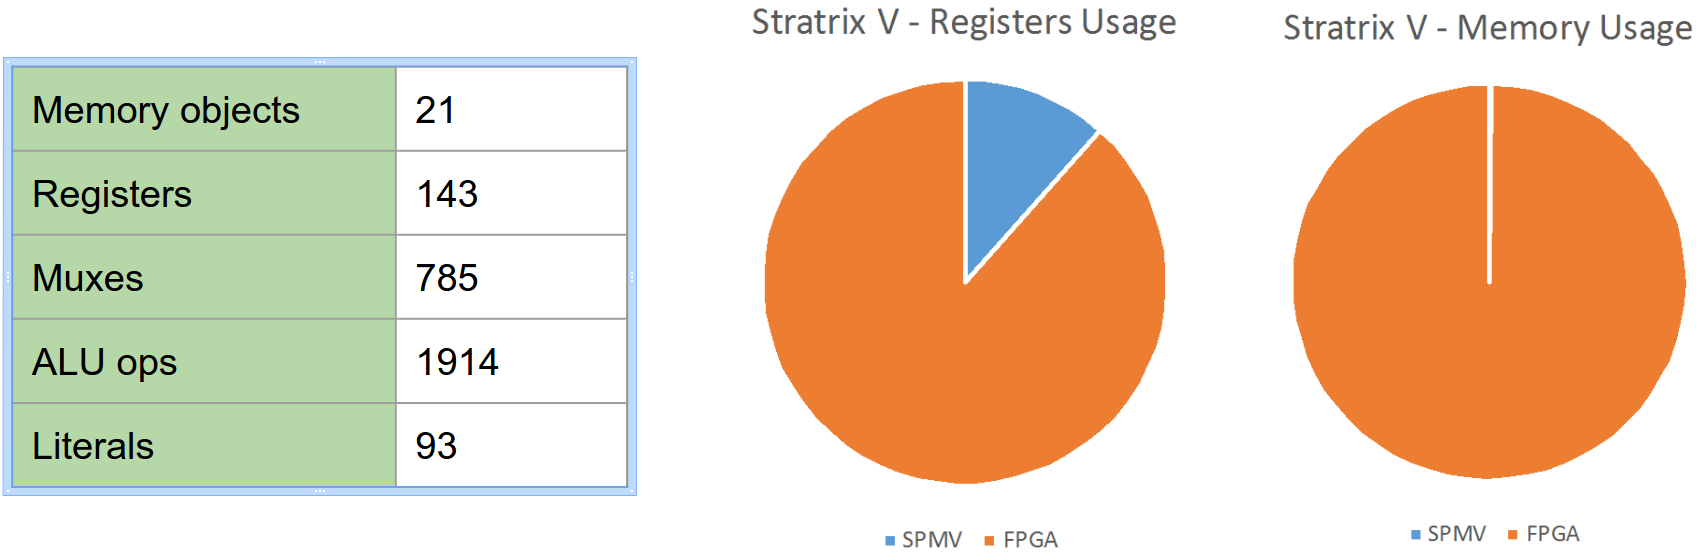
\includegraphics[width=0.5\textwidth]{figures/hardware_cost}
\caption{Cocoh's hardware cost evaluation}
\label{fig:hardware_cost}
\end{figure}

In summary, FlexGraph current average performance is 0.1 Gflops (using the lower bound of the largest dataset in our experiment). This is in part with our HLS implementation of the same kernel. We have identified several optimization opportunities to boost the accelerator performance.\\
We added some performance counters into FlexGraph accelerator to monitor the memory stalls in each processing elements and identify bottlenecks. Figure \ref{fig:memory_stalls} shows the memory stalls distribution over three datasets \textit{m8}, \textit{m10} and \textit{m12}. The blue region represents the execution cycles, the orange region represents the stall cycles occurring when we access the matrix column indices, this is \textit{coldata} buffer in the SPMV speudo-code (line 4 in listing 1). The gray region represents the stall cycles when accessing the vertices active masks (line 6 in listing 1). We can significantly reduce the stall cycles by prefetching the blocks before they are needed to hide the memory latency. Using a simple next-line prefetcher will suffice since we know the access pattern on \textit{coldata}.\\
Another performance optimization is in reducing the impact of the branch operation when checking if a vertex is active of not (line 7 in listing 1). We will investigate adding a preliminary test on the entire 32-bit mask to see if it is zero and skip the whole block altogether.\\ 
Lastly, another performance opportunity is increasing the number of precessing elements. Figure \ref{fig:single_core_perf} showed the performance gain of using two cores versus a single one. Having multiple processing elements will improve the system memory level parallelism by overlapping the execution of some processing element while others are stalled on memory accesses. We ran some estimate of the current design hardware cost using Cocoh's framework (see Figure \ref{fig:hardware_cost}) and it showed that our memory usage is very small (about 1\% of the target Stratix V FPGA capacity). Also, FlexGraph accelerator only currently consumes 15\% of the registers capacity. With this reserve, we anticipate extending the number of processing elements to 16. A challenge that we will have to resolve when adding additional processing elements is the synchronization of write accesses for the active masks. Another challenge will be the arbitration latency in the LSU when communicating with all nodes,    since the single LSU will now become a bottleneck in the system.